% THIS IS SIGPROC-SP.TEX - VERSION 3.0
% WORKS WITH V3.1SP OF ACM_PROC_ARTICLE-SP.CLS
% JUNE 2007
%
% It is an example file showing how to use the 'acm_proc_article-sp.cls' V3.1SP
% LaTeX2e document class file for Conference Proceedings submissions.
% ----------------------------------------------------------------------------------------------------------------
% This .tex file (and associated .cls V3.1SP) *DOES NOT* produce:
%       1) The Permission Statement
%       2) The Conference (location) Info information
%       3) The Copyright Line with ACM data
%       4) Page numbering
% ---------------------------------------------------------------------------------------------------------------
% It is an example which *does* use the .bib file (from which the .bbl file
% is produced).
% REMEMBER HOWEVER: After having produced the .bbl file,
% and prior to final submission,
% you need to 'insert'  your .bbl file into your source .tex file so as to provide
% ONE 'self-contained' source file.
%
% Questions regarding SIGS should be sent to
% Adrienne Griscti ---> griscti@acm.org
%
% Questions/suggestions regarding the guidelines, .tex and .cls files, etc. to
% Gerald Murray ---> murray@acm.org
%
% For tracking purposes - this is V3.0SP - JUNE 2007

% \documentclass{acm_proc_article-sp}
\documentclass{sig-alternate}

\graphicspath{{figures/}}

% Alter some LaTeX defaults for better treatment of figures:
    % See p.105 of "TeX Unbound" for suggested values.
    % See pp. 199-200 of Lamport's "LaTeX" book for details.
    %   General parameters, for ALL pages:
    \renewcommand{\topfraction}{0.9}	% max fraction of floats at top
    \renewcommand{\bottomfraction}{0.8}	% max fraction of floats at bottom
    %   Parameters for TEXT pages (not float pages):
    \setcounter{topnumber}{2}
    \setcounter{bottomnumber}{2}
    \setcounter{totalnumber}{4}     % 2 may work better
    \setcounter{dbltopnumber}{2}    % for 2-column pages
    \renewcommand{\dbltopfraction}{0.9}	% fit big float above 2-col. text
    \renewcommand{\textfraction}{0.07}	% allow minimal text w. figs
    %   Parameters for FLOAT pages (not text pages):
    \renewcommand{\floatpagefraction}{0.7}	% require fuller float pages
	% N.B.: floatpagefraction MUST be less than topfraction !!
    \renewcommand{\dblfloatpagefraction}{0.7}	% require fuller float pages

	% remember to use [htp] or [htpb] for placement


\begin{document}

\title{Software Trajectory Analysis:\\An empirically based method for automated software process discovery}

%\numberofauthors{8} %  in this sample file, there are a *total*
% of EIGHT authors. SIX appear on the 'first-page' (for formatting
% reasons) and the remaining two appear in the \additionalauthors section.
%
\numberofauthors{1}
\author{
% You can go ahead and credit any number of authors here,
% e.g. one 'row of three' or two rows (consisting of one row of three
% and a second row of one, two or three).
%
% The command \alignauthor (no curly braces needed) should
% precede each author name, affiliation/snail-mail address and
% e-mail address. Additionally, tag each line of
% affiliation/address with \affaddr, and tag the
% e-mail address with \email.
%
% 1st. author
\alignauthor Pavel Senin \\
%\titlenote{Corresponding author. Email: senin@hawaii.edu}\\
	\affaddr{IRISA, campus de Beaulieu}\\
	\affaddr{35042 Rennes Cedex, France}\\
	\email{pavel.senin@inria.fr}\\
% 2nd. author
%\alignauthor Philip M. Johnson \titlenote{PhD Thesis adviser.}\\
%	\affaddr{CSDL, University of Hawaii at Manoa}\\
%	\affaddr{1680 East-West Rd, Honolulu, HI 96822}\\
%	\email{johnson@hawaii.edu}
}
% There's nothing stopping you putting the seventh, eighth, etc.
% author on the opening page (as the 'third row') but we ask,
% for aesthetic reasons that you place these 'additional authors'
% in the \additional authors block, viz.
%\additionalauthors{Additional authors: John Smith (The Th{\o}rv{\"a}ld Group,
%email: {\texttt{jsmith@affiliation.org}}) and Julius P.~Kumquat
%(The Kumquat Consortium, email: {\texttt{jpkumquat@consortium.net}}).}
%\date{30 July 1999}
% Just remember to make sure that the TOTAL number of authors
% is the number that will appear on the first page PLUS the
% number that will appear in the \additionalauthors section.
\maketitle
\begin{abstract}
A process defines a set of routines which allow one to organize, manage and improve activities in order to reach a goal. With expert intuition and a-priori knowledge, software processes have been modeled for a long time, resulting in the Waterfall, Spiral and other development models. Later, with the wide use of SCM \footnote{Software Configuration Management} systems and the public availability of primitive software process artifact trails \footnote{software roadmaps, bug and issue tracking and management systems, public mailing lists}, formal methods such as Petri Nets, State Machines and others have been applied to the problem of recurrent process discovery and control. Recent advances in metrics effort, increased use of continuous integration, and extensive documentation of the performed process make information-rich fine-grained software process artifacts trails available for analysis. This fine-grained data has the potential to shed new light on the software process. In this work I propose to investigate an automated technique for the discovery and characterization of recurrent behaviors in software development - ``programming habits'' either on an individual or a team level.
\end{abstract}

% A category with the (minimum) three required fields
%\category{H.4}{Information Systems Applications}{Miscellaneous}
%A category including the fourth, optional field follows...
%\category{D.2.8}{Software Engineering}{Metrics}[complexity measures, performance measures]

%\terms{Software process}

%\keywords{ACM proceedings, \LaTeX, text tagging} % NOT required for Proceedings

\section{Introduction and Motivation}
A \textit{software process} is a set of activities performed in order to design, develop and maintain software systems. Examples of such activities include design methods; requirements collection and creation of UML diagrams; testing and performance analysis. The intent behind a software process is to structure and coordinate human activities in order to achieve the goal - deliver a software system successfully. 

Much work has been done in software process research resulting in a number of industrial standards for process models (CMM, ISO, PSP etc. \cite{citeulike:5043104}) which are widely accepted by many governmental and industrial institutions. Nevertheless, software development remains error-prone and more than a half of all software development projects end up failing or being very poorly executed. Some of them are abandoned due to running over budget, some are delivered with such low quality or so late that they are useless, and some, when delivered, are never used because they do not fulfill requirements \cite{citeulike:7351135}. The cost of this lost effort is enormous and may in part be due to our incomplete understanding of software process.

There is a long history of software process improvement through proposing specific patterns of software development. For example, the Waterfall Model process proposes a sequential pattern in which developers first create a Requirements document, then create a Design, then create an Implementation, and finally develop a Test. Alternatively, the Test Driven Development process proposes an iterative pattern in which the developer must first write a test case, then write the code to implement that test case, then re-factor the system for maximum clarity and minimal code duplication \cite{citeulike:2703162}. A significant problem with this traditional top-down approach to process development is that it requires the developer or manager to notice a recurrent pattern of behavior in the first place \cite{citeulike:5043104}. Another weakness of this approach is that such models are often normative and influenced by individual perception - they prescribe what should be done instead of describing the actual process \cite{citeulike:2678511}.

As an alternative to the top-down approach in my research, I am applying knowledge discovery and data mining techniques to the domain of software engineering in order to evaluate their ability to automatically notice interesting recurrent patterns of behaviors from collected software process artifacts. While I am not proposing to be able to infer a complete and correct software process model, my system will provide its users with a formal description of recurrent behaviors in their software development. As a simple example, consider a development team in which committing code to a repository triggers a build of the system. Sometimes the build passes, and sometimes the build fails. To improve the productivity of the team, it would be useful to be aware of any recurrent behaviors of the developers. My system might generate one recurrent pattern consisting of a) implementing code b) running unit tests, c) committing code and d) a passed build: $i \rightarrow u \rightarrow c \rightarrow s $, and another recurrent pattern consisting of a) implementing code, b) committing code, and c) a failed build: $i \rightarrow c \rightarrow f $. The automated generation of these recurrent patterns can provide actionable knowledge to developers; in this case, the insight that running test cases prior to committing code reduces the frequency of build failures.

\section{Relevant prior work}
Although process mining in the business domain is a well-established field with much software developed up to date (ERP, WFM, SCM, CRM and other systems), ``Business Process Intelligence'' tools usually do not perform process discovery and typically offer relatively simple analyses that depend upon a correct a-priori process model \cite{citeulike:5044991} \cite{citeulike:3718014} \cite{citeulike:2678511}. This fact restricts direct application of business domain process mining techniques to software engineering, where processes are usually performed concurrently by many agents, are much more complex, and typically have a higher level of noise. Taking this fact into account, I will review only the approaches to the process (or workflow) mining for which applicability to software process was expressed. 

Perhaps, the research most relevant to my own was done by Cook \& Wolf in \cite{citeulike:328044}. The authors developed \textit{``process discovery''} techniques intended to discover process models from event streams. The authors did not attempt to generate a complete model, but rather to generate sub-models that express the most frequent patterns in the event stream. They designed a framework that collects process data from history logs, and generates a set of recurring patterns of behavior characterizing observed process. In this work they extended two methods of \textit{grammar inference} from previous work: purely statistical (neural network based \textit{RNet}) and purely algorithmic (\textit{KTail}) as well as developed their own Markovian method (\textit{Markov}). 

\begin{figure}[htp]
   \centering
   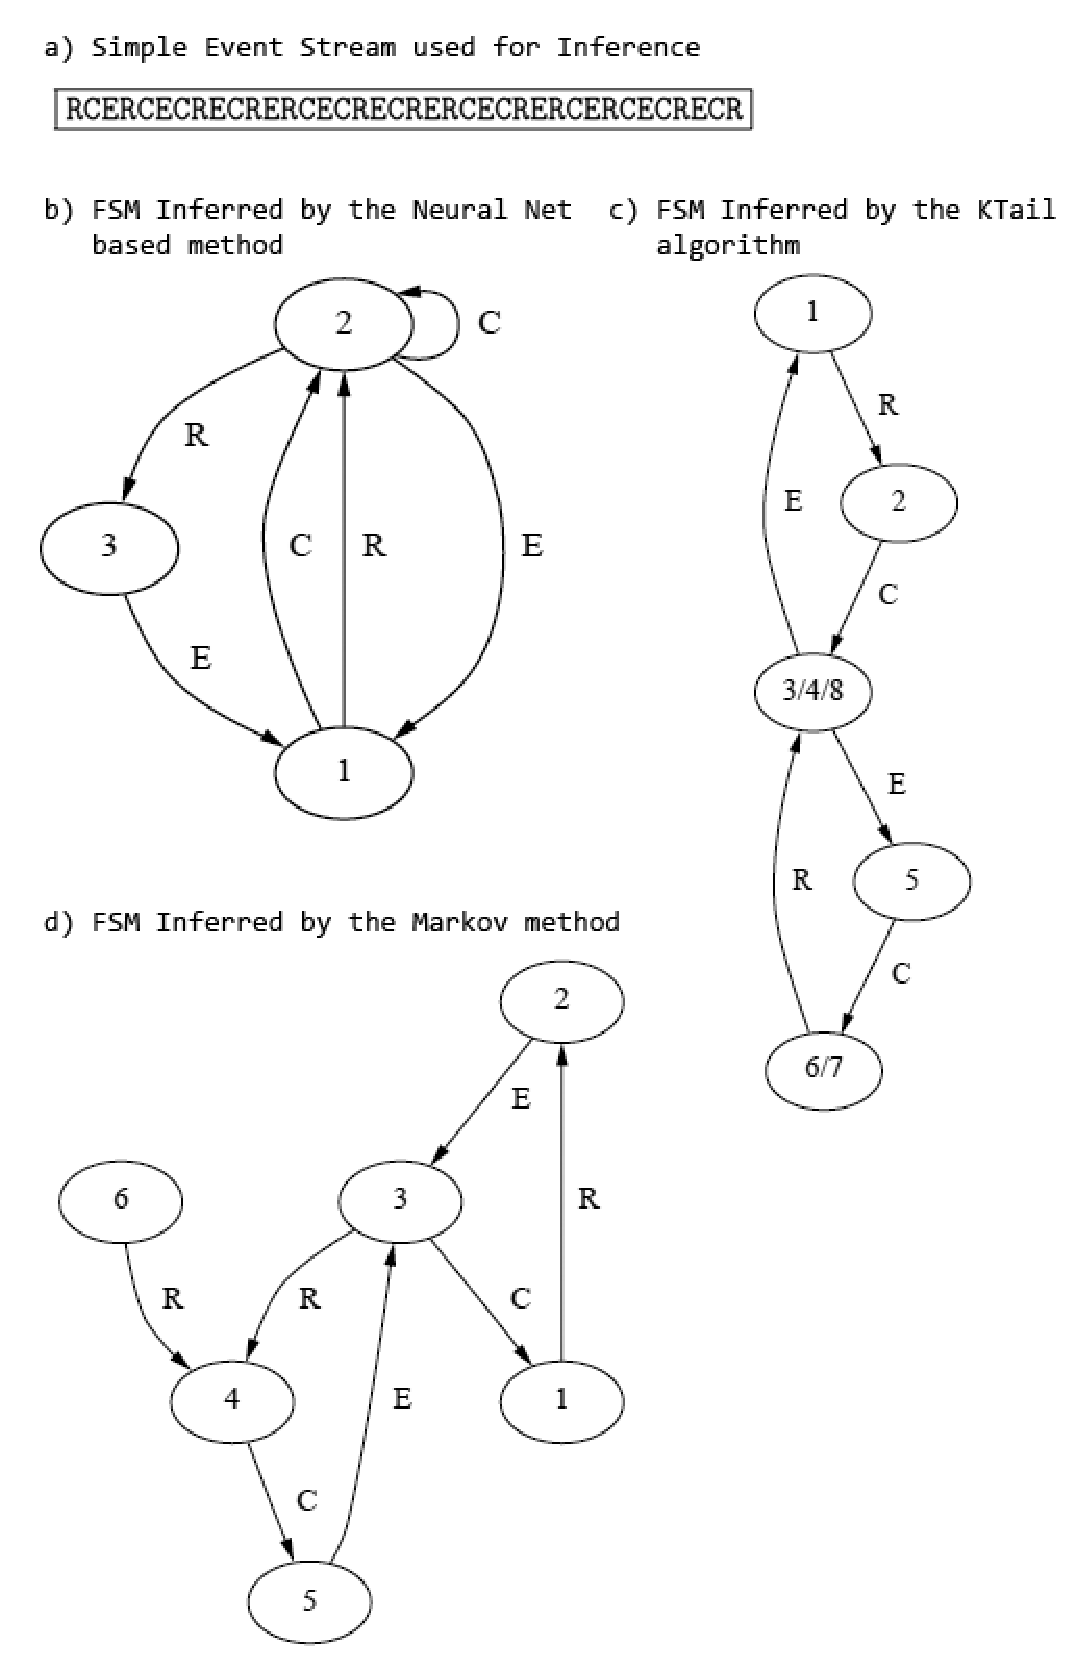
\includegraphics[height=132mm]{inference.eps}
   \caption{Process discovery through the grammar inference: panel a) a sample event stream (simple process involving three types of events: Edit, Review, and CheckIn); and FNA results obtained by applying three methods of process discovery from Cook \& Wolf \cite{citeulike:328044}.}
   \label{fig:inference}
\end{figure}


The first method extended by the authors, the neural-network based grammar inference, RNet algorithm, defines a recurrent neural network architecture which is trained by the sequences of events. After training, this neural net is able to characterize a current system state by looking on past behavior. The authors extract the FSM from the trained neural network by presenting different strings to it and extracting the hidden neurons activity through observations. Due to the nature of Neural Net, closely related activation patterns are clustered into the same state; therefore, by noting the current pattern, the input token, and the next activation pattern, transitions are recorded and compiled into the inferred FSM.

The second method investigated, is a purely algorithmic KTail method, which was taken from the work of Biermann \& Feldman \cite{citeulike:5120603}. The idea is that a current state is defined by what future behaviors can occur from it. The \textit{future} is defined as the set of next $k$ tokens. By looking at a window of successor events, the KTail algorithm can build the equivalence classes that compose the process model. The authors extensively modified the original KTail algorithm improving the folding in the mined model making it more robust to noise.

The Markov based method developed by the authors is based on both algorithmic and statistical approaches. It takes to account past and future system behavior in order to guess the current system state. Assuming that a finite number of states can define the process, and that the probability of the next state is based only on the current state (Markov property), the authors built a $n^{th}$-order Markov model using the first and second order probabilities. Once built, the transition probability table corresponding to the Markov model is converted into FSM which is in turn reduced based on the user-specified cut-off threshold for probabilities.

The authors implemented all three of these algorithms in a software tool called \textsc{DaGama} as a plugin for larger software system called Balboa \cite{citeulike:5120757}. By performing benchmarking, Cook \& Wolf found that the Markov algorithm was superior to the two others. RNet was found to be the worst of the three algorithms. The software tool was applied to a real-world process data and demonstrated an abstraction of the actual process executions and ability to capture important properties of the process behavior. The major backdraw of the approach, as stated by the authors, lies in the inability of the FSMs to model concurrency of processes which limits its applicability to the software development process. Later, Cook et al. in \cite{citeulike:5128143} addressed this limitation by using Petri-nets and Moore-type FSM.

Another set of findings relevant to my research approach was developed by Rubin et al. \cite{citeulike:1885717} and van der Aalst et al. \cite{citeulike:3718014} and is called \textit{incremental workflow mining}. The authors not only designed sophisticated algorithms but built a software system using a business process mining framework called ProM by van Dongen et al. \cite{citeulike:5043673} which synthesizes a Petri Net corresponding to the observed process. The system was tested on SCM logs and while the process artifacts retrieved from the SCM system are rather high-level, the approach discussed is very promising for the modeling of software processes from the low-level product and process data.

The algorithm input is an event chain constructed through the ``abstraction on the log level'', which aggregates basic events into single high-level entities, is treated with the \textit{Generate} part of the \textit{``Generate and Synthesis''} \cite{citeulike:3718014} algorithm in order to generate a \textit{Transition System} which represents an ordered series of events. This algorithm looks at the history (prefix) and the future (suffix) sequences of events related to the current one in order to discover transitions.  When applied to the abstracted log information, the algorithm generates a rather large Transition System graph where edges connect to abstracted events. This transition system is then successively simplified by using various reduction strategies. At the last step of the incremental workflow mining approach, Transition Systems are used to \textit{Synthesize} labeled Petri nets (where different transition can refer to the same event) with the help of \textit{``regions theory''} \cite{citeulike:5128170}. As with the Transition System generation, the authors investigate many different strategies of Petri nets synthesis, showing significant variability in the results achieved. (see Figure \ref{fig:petri}). The significant contribution of this research is in the generality of the method. It was shown that by tuning the ``Generate'' and ``Synthesize'' phases it is possible to tailor the algorithm to a wide variety of processes. In particular, as mentioned before, Rubin et al. successfully applied this framework to the SCM logs and audit trails analysis.

The work by Cook \& Wolf and van der Aalst et al. was recently built upon by Huo et al. \cite{citeulike:7690766} \cite{citeulike:7691059}. The authors follow previous attempts by implementation of a software process pattern-mining engine built upon Petri Nets. The patterns discovered by its application fully or partially compose an ``enactment model'' which in turn are compared one by one with a set of pre-defined software process models provided by an expert. By introducing the means for measure of enactment model deviation from templates authors are able to evaluate its fitness and provide recommendations for software process improvements or template model adjustment. While such results are highly valuable within industrial settings, the authors agreed that an inability to discover and formalize novel patterns as well as low tolerance for noise are among the limitations of their approach.

In addition to the above, the latest trends in software process research emphasize mining of software process artifacts and behaviors \cite{citeulike:2678511} \cite{citeulike:5043664} \cite{citeulike:5112229}. 

It is worth noting here that while reviewed work demonstrate general approaches to modeling of concurrent processes, to the best of my knowledge their application to the real world data was very limited. This may be partially due to the high level of noise and computational limitations which made inferring complete models too complex and impractical to use; or maybe due to the lack of the means to collect fine-grained software process artifacts which made models too abstract.

In my approach I am planning to address both issues by leveraging the ability of the Hackystat system \cite{citeulike:4041809} to collect fine grained data and by the application of advanced symbolic and temporal data mining techniques which are both efficient and resistant to noise.

\begin{figure}[htpb]
   \centering
   \includegraphics[height=40mm]{petri.eps}
   \caption{Illustration of the ``Generation and Synthesis Approach'' from \cite{citeulike:5043673}: a) Transition System with regions shown; b),c) Petri Nets synthesized from the Transition System.}
   \label{fig:petri}
\end{figure}

\section{Research objectives}
As shown by previous research, it is possible to infer and successively formalize sequential software process by observing its artifacts, and in particular, recurrent behavioral patterns. The problem of finding such patterns is the cornerstone of my research. Solving this will extend previous research with a new knowledge that will support improvements in our understanding of software process.

The main research objectives of my work is to design, develop and evaluate a previously unexplored approach to discovering recurrent behaviors in software process through the data mining of low-level process and product artifacts. To reach this goal I am planning to perform the following steps. 

First I am exploring the applicability of proposed pattern-mining techniques to various levels of software process artifacts complexity. This exploratory study will result in a set of well-defined data mining workflows designed for particular kinds and coarseness of software process data and research goals. 

Secondly, implementations of these workflows will constitute the core of the Software Trajectory package aiding recurrent behavior discovery. This software will be a stand-alone database-backed framework which provides users with ability to design and use arbitrary filters in order to shrink the amount of reported patterns by specifying events of interest, their order or their origin.  

Finally, the approach implemented in this software system will be empirically evaluated. I plan to perform the evaluation on three types of data sets which differ by their origin and complexity: the first data set will consist of the events collected by Hackystat from a directed development process in a controlled environment - a classroom development project. The second data set will consist of a data collected from an open-source project; while the third data set will originate from a large-scale industrial software development project. 

\section{Research approach}
My approach to this problem rests on the application of data-mining techniques to symbolic time-point and time-interval series constructed directly from the software process artifacts such as SCM logs, software audit trails or telemetry streams provided by Hackystat or by a similar in-process software development monitoring system.

To investigate the requirements for a software tool that aids in the discovery of recurrent behavioral patterns in software process, I am designing and developing the ``Software Trajectory'' framework. A high-level overview of the framework is shown in Figure \ref{fig:system_overview} and resembles the flow of the ``Knowledge Discovery in Database'' process discussed by Han et al. in \cite{citeulike:709476}. As shown, the data collected by Hackystat is transformed into an intermediate symbolic format and then indexed for further use in data-mining. The tools, designed for data-mining, have a specific restrictions placed on the search space by domain and context knowledge in an attempt to limit the amount of reported patterns to useful ones. I am planning to design a GUI in a way that will allow easy access and modification of these restrictions.

While I plan to use Hackystat as a primary data collection system in my future experimental setup, for the current exploratory study I am working with various ways of data collection, extraction and abstraction. The ability to abstract into symbolic representation various software artifact streams such as SCM logs and audit trails is crucial for the exploratory study phase enabling me to experiment with much broader spectrum of existing software process data collections.

\section{Data and analysis methods}
Various types and complexity of data are available for software process analysis. For example, simple data extracted from SCM logs allow us to track software change and to perform a basic software process reconstruction and modeling - however a very little information can be recalled about individual development activities and behaviors from such models. When development audit trails added to analyzes, the enriched data allow us to shed more light on the performed process. By using a contemporary automated build system and code analysis tools it is possible to collect a much broader spectrum of process artifacts and software metrics. Moreover a centralized build system creates a set of singular time points which are persisting through and tying together processes performed concurrently by developers allowing concurrent process reconstruction. Finally, collecting temporal data about atomic development events by the means of Hackystat and similar systems - such as results of background compilation and unit tests, IDE buffer transfers etc. along with quantification of the development effort enables characterization of the dynamic behavior of software process in great detail. However, rich data brings much more noise \footnote{The term \textit{noise} here is used to refer to many types of discrepancy between logged data and performed process: incomplete logs, incorrectly logged events, human or technical errors etc. If not handled properly, the noise distorts process reconstruction making models useless, as shown in \cite{citeulike:2678511}.} which makes process analysis a non-trivial task.  

To overcome the noise and computational complexity issues I have turned to recent advances in two research fields: patterns mining from temporal data and patterns (motifs) discovery in genetics. Within both fields researchers work with vast amounts of the data on a daily basis and many new methods have been developed which are characterized by their efficiency, computational simplicity and high noise tolerance. The data-mining techniques employed in these fields are based on the mining of the symbolic data, and while in Bioinformatics DNA and AA sequences (proteins) historically represented by symbols, in the temporal data mining some preliminary conversion is required \cite{citeulike:2821475}. By following this model in my approach I am also performing two steps: at first software process artifacts trails are reduced to a symbolic form and later this data is indexed and mined for recurrent patterns.

\begin{figure}[tpb]
   \centering
   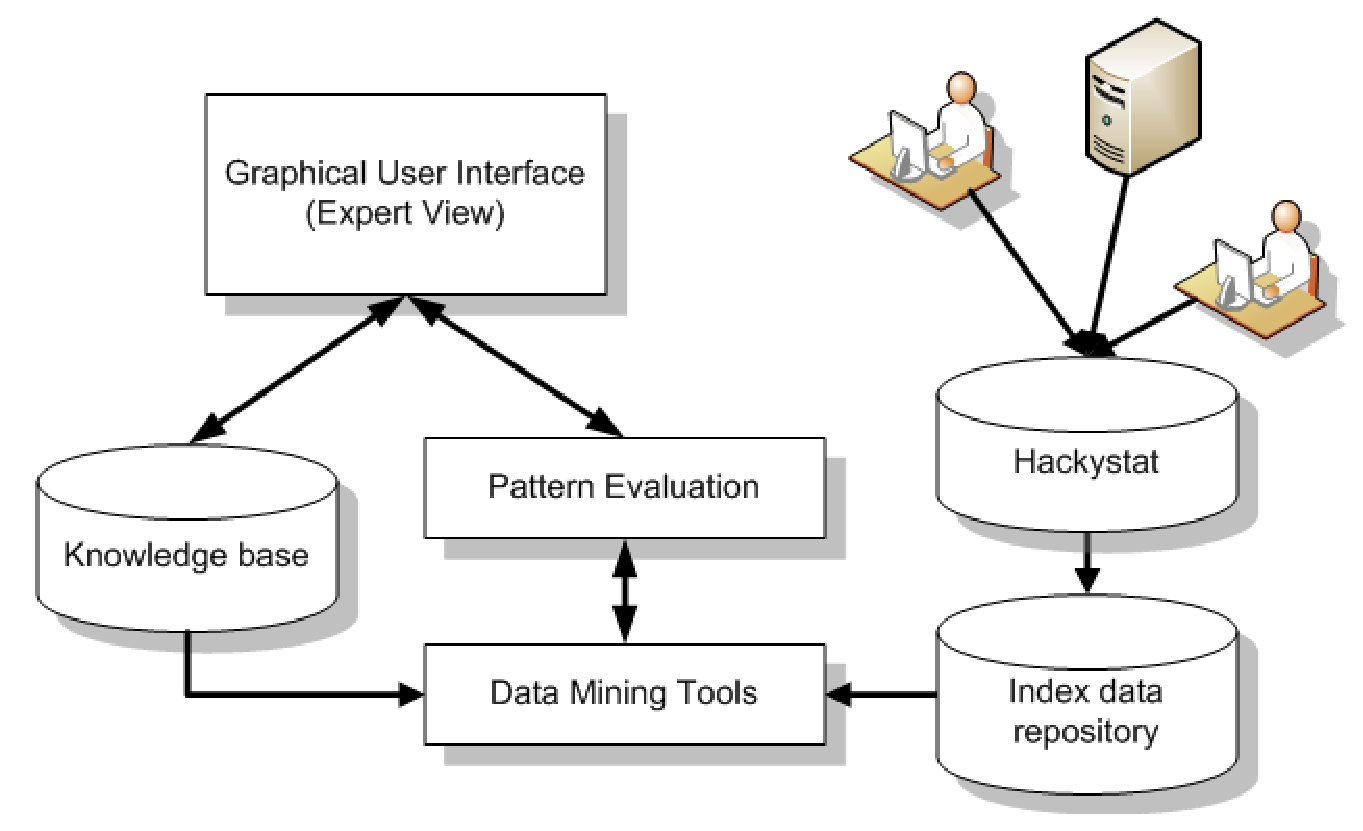
\includegraphics[height=50mm]{system_overview.eps}
   \caption{The high-level system overview. Software engineering process and product data are collected and aggregated by Hackystat and then used to generate temporal symbolic indexes. Data mining tools constrained by software engineering domain knowledge are then used for unsupervised patterns discovery. The GUI provides an interface to the discovered patterns and aids in investigation of a discovered phenomena.}
   \label{fig:system_overview}
\end{figure}

\subsection{Application of the symbolic aggregate approximation.}
The current state of the art approach in temporal data mining is called Symbolic Aggregate approXimation and was proposed by Lin et al. in \cite{citeulike:2821475}. This method extends the PAA-based approach, inheriting algorithmic simplicity and low computational complexity, while providing satisfactory sensitivity and selectivity in range-query processing. Moreover, as mentioned by the authors, the use of a symbolic representation opens the door to the existing wealth of data-structures and string-manipulation algorithms in computer science such as hashing, regular expression pattern matching, suffix trees etc. As showed by the authors, SAX outperforms all previously known methods - DFT, DWT, DTW and similar - by using SAX it is possible to index and find discords - recurrent and ``surprise'' patterns in vast amounts of data in almost linear time and space \cite{citeulike:1630245} \cite{citeulike:3025877} \cite{citeulike:3000416}. 

Previously in my research I have attempted to mine behavioral patterns from software telemetry streams by using DTW (similarly to the speech recognition) and application of SAX was a natural continuation of this attempt, however the results of such application were not encouraging as shown further in Section \ref{results}. While resolving issues and evaluating parameters for SAX-performed data reduction I have noticed that due to the PAA step of the algorithm a high level of noise in the raw data can be dramatically reduced  leaving only a major time-series trends for successful ``symbolization''. In my opinion, this protocol can be adopted for the complexity reduction of the software process artifacts streams. For example, if symbolic coding of a performed software process would be $d \rightarrow d \rightarrow d \rightarrow u \rightarrow d \rightarrow d \rightarrow d \rightarrow u \rightarrow c \rightarrow s $ inferring a long cycle of development with intermediate unit test at some point (position 4) succeeded by a unit test, commit and build success, it may be necessary to dismiss this intermediate unit test event and collapse in time all development events into the single one, transforming the original sequence into $d \rightarrow u \rightarrow c \rightarrow s $ and thus reducing the pattern complexity. The implementation of this approach is currently under way and will be included within my exploratory study.

\subsection{Application of motif mining in biological data.}
Multiple alignments of protein sequences are important in many biological applications including phylogenetic tree estimation, secondary structure prediction and critical residue identification. In multiple alignment algorithms gaps and substitution usually introduced within possibly similar sequences in order to find the best possible score for an alignment, clever weighting of such discrepancies was shown to improve alignments. Further, recent advances in MSA (multiple sequence alignment) algorithms \cite{citeulike:692} include a new method for design and evaluation of objective functions for improving alignments by its profiling by statistically inferred weighting schema. Such a heuristic strategy can be also adopted within the search of ``software development motifs'' - for example in an attempt to reduce complexity one may ignore (score low) the presence or lack of code analysis events within a development cycle. This will immediately align together patterns with or without such events, making them statistically much more noticeable while preserving the overall contextual correctness.

\begin{figure}[ht]
   \centering
   \includegraphics[height=140mm]{dev_clustering_vertical.eps}
   \caption{Clustering of developers behavior using symbolic approximation and temporal motif frequencies vectors. This analysis captured similar development behavior among developers. Developers \#2 and \#7 were consistent (no bursts observed) in both, coding and measuring effort during whole time interval, while all others can be characterized with bursty, inconsistent effort.}
   \label{fig:cluster_developers}
\end{figure}

Another idea seen in both methods which can be borrowed is the clever distance function implementation - it will score sequences different by a single symbol (single substitution) as equal if the both symbols are approximately equal to each other in the context of actions. By adopting this strategy one may consider events representing running code analysis tools such as CheckStyle, PMD, FindBugs (all are Java code analysis tools) and SCLC (code line counter) as equal in their meaning and if the sequences representing software process are different only by these events, than no value will be added to the resulting distance.

\section{Preliminary results}\label{results}
During my work on the pilot version of Software Trajectory framework, I began a set of small exploratory experiments in order to aid in the architectural design, data-mining algorithms selection and implementation. In addition, these experiments helped me to outline the boundaries of applicability of my approach to certain problems in software engineering. I call these experiments the \textit{Pilot study}.

One of the Pilot study experiments was performed in order to evaluate the ability of SAX approximations and indexing to capture a temporal specificity of telemetry streams through the discovery of temporal motifs - recurrent temporal patterns. The goal of the experiment was to cluster developers by their development behaviors and to find correlations between software metrics streams. Knowing about the frequently misleading results of a time-series clustering \cite{citeulike:227029}, I did not expect to capture many interesting facts, nevertheless the results were encouraging. The data used in this study were collected from eight students and represent Hackystat metrics collected during sixty days of a classroom project. The streams under analysis were composed by quantifying development events within a day: for example for the BuildSuccess stream a single value 5 means that five builds succeeded within that day. 

The two clustering experiments were conducted using the distance between motif frequencies vectors (note that temporal ordering of motifs was not accounted in these analysis) extracted by indexing of telemetry streams. The procedure for building such vectors closely follows SAX approximation and uses a sliding window to extract all subsequences (potential motifs) from a given stream. These subsequences are mapped into strings and stored in the hash-like structure. At the next step the hash entries are counted and sorted by the frequency of occurrence. The vector of $N$ most frequent motifs then used in the clustering.

\begin{figure}[htpb]
   \centering
   \includegraphics[height=180mm]{telemetry_streams.eps}
   \caption{Aggregated Telemetry streams for classroom pilot dataset presenting non-cumulative values for each metrics for 60 days.}
   \label{fig:streams}
\end{figure}

At first, by clustering of development time telemetry streams collected from individual developers I was able to group developers with similar behavioral patterns within clusters, which indicates the feasibility of the classification by effort approach. Figure \ref{fig:cluster_developers} depicts results of this analysis.

However clustering of product-related telemetry streams was not successful. I was able to group telemetry streams, but while these groups look intuitively meaningful - for example clustering together filemetrics and development time - the close examination of the stream features suggests that this grouping happened due to the similar temporal behavior on the short stretches rather then positive correlation. This result, while proving the correctness of approach, indicates its limitation, pointing out that instead of using just motif frequencies, some temporal ordering should be taken into account. Figure \ref{fig:cluster_streams} displays the results of this analysis.

Another result within a Pilot Study was also achieved by the direct application of SAX indexing. For this experiment I used data collected from my own concurrent development of Trajectory software package and JMotif library. Within a symbolic approximation paradigm the change of symbols can be interpreted as growth or drop in the value of underlying data stream: for example consecutive $ab$ symbols indicate that growth happened and $ba$ correspond to a drop. The idea was to find if there was any recurrent drop or growth events coincidence within two streams. For this purpose I defined a sliding window consisting of three days and searched for such coinciding within the window events. Events were found in the development time stream, churn, commit and others. Detailed analysis of coinciding growth events revealed that changes within JMotif data manipulation routines almost always followed by changes within Trajectory data analyzes routines which are heavily relying on the JMotif API. While within my two-project software portfolio such a discovery is a quite obvious fact, one can see an immediate application of this method to a large software projects portfolio or a large software system where it will be possible to build a repertoire of frequent consecutive changes aiding in estimate of an effort required for performing certain changes.

\section{Exploratory study directions}
The previous section describes two completed experiments which provide an insight into the applicability of SAX approximation of Telemetry streams to discovery of recurrent behaviors in software process. Work on both experiments resulted in a database schema which supports symbolic indexing of telemetry streams. Such storage solution provides an immediate and structured access to the symbolic streams allowing to perform time-range queries with use of regular expressions (in SQL language) and to extract sequences of interest which for example include successful Unit-Test, or Commit events, or software metrics values above an arbitrary threshold. This database-driven solution is somewhat similar to the CVSAnalY tool \cite{citeulike:6544724} providing an abstraction layer over the raw, mostly unstructured data. One of the direction I am working on right now is the complimentary use of both databases under unifying API in order to evaluate a capacity of such approach in the recurrent behavior discovery for the MSR challenge \cite{citeulike:5043676}.

As mentioned before, motif finding in protein sequences is a well-established research field which deals with vast amount of data as well as with high level of noise. This noise problem is inevitable in biology and reflects a natural way of evolution in life through mutations. Recent advances in biological data mining resulted in a wealth of algorithms and software tools.  According to \cite{citeulike:964046} there are two categories of approaches for motif finding in biological sequences: while the first one is based on the similar to reviewed concepts such as HMM and automata, the second category ``uses patterns with `mismatch representation' and define a signal to be a consensus pattern allowing up to a certain number of mismatches to occur in each instance of the pattern''. This second approach looks like a very promising alternative to previously explored directions in process mining while extending the exact motifs search approach explained before. Allowing mismatches in the noise from non-frequent events will not decrease the evidence value for the similar patterns, allowing us to identify key events of the observed process (as similar to the key amino-acids residues within protein sequences). I am planning to perform an experiment consisting of abstraction of software process artifacts into the symbolic representation mimicking protein encoding and application of motif-finding packages with purpose of evaluation of their ability to recall frequent patterns from such data.

\begin{figure}[ht]
   \centering
   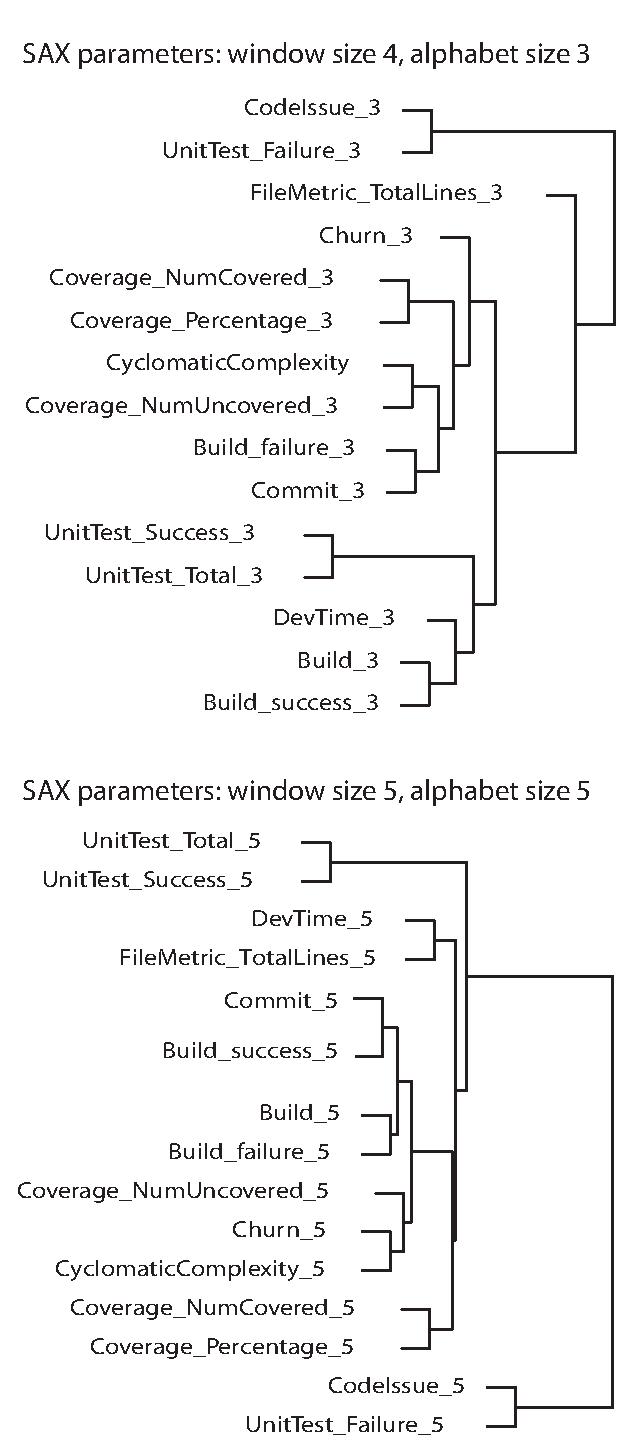
\includegraphics[height=165mm]{streams_clustering.eps}
   \caption{Clustering of telemetry streams for classroom pilot dataset using symbolic approximation and vectors of motif frequencies. While it seems to be meaningful to find correlation between \textit{UnitTest\_Failure} and \textit{CodeIssue} streams unit test, this grouping happened due to the similarity of behavior pattern - short, high amplitude bursts; but note, there is no correlation of features in time. There are two trees for different SAX parameters shown to display inconsistency of clustering.}
   \label{fig:cluster_streams}
\end{figure}

Concurrent software processes occur within a team working on a common goal. Within such processes developers interact at many levels by means of various software tools such as SCM, bug and issue tracking systems, e-mails etc. In the context of my exploratory study I am going to put the research focus on the role of build automation (such as continuous integration) and its ability to serve as a place which persists among all processes providing means of interaction for all participating agents and potentially influencing their individual behaviors. I plan to perform data mining analyzes on intervals of continuous telemetry streams collected from individual agents using automation-created events as time points breaking these streams onto intervals. I expect to find behavioral specificity within such fragments reflecting different phases of development (such as bug-fixing, testing or a ``death march'') as well as differences among sets from individual agents reflecting team-assigned roles.

\section{Future empirical study design}
I propose to conduct two case studies: \textit{Public data case study}, and \textit{Classroom case study} in order to empirically evaluate the capabilities and performance of Software Trajectory framework. These studies differ in the granularity of data used, and in the approaches for evaluation. 

My intent behind these empirical studies is to assess the ability of Software Trajectory framework to recognize well known recurrent behavioral patterns and software processes (for example Test Driven Development), as well as its ability to discover new ones. In addition, these studies will support a classification and extension of the current Hackystat sensor family in order to improve Software Trajectory's performance. It is quite possible that some of the currently collected sensor data will be excluded from the Software Trajectory datasets, while some new ones will be designed and developed in order to capture important features from the studied software development data streams. 

The proposed public data case study is based on the use of publicly available Software Configuration Management (SCM) audit trails of the big, ongoing software projects such as Eclipse, GNOME etc. Mining of SCM repositories is a well-developed area of research with much work published \cite{citeulike:5043676}. SCM repositories contain coarse software product artifacts which are usually mined with a purpose of discovering of various characteristics of software evolution and software process. I am using a mixed-method approach in this study. In the first phase of this study, I plan to perform SCM audit trail data mining following published work and using Software Trajectory as a tool in order to discover confirmed patterns in software process artifacts, and thus quantitatively evaluate Software Trajectory's performance when compared to existing tools. In the second phase, I will develop my own pre-processing and taxonomy mapping of software process artifacts into temporal symbolic series. By using this data and Software Trajectory framework, I plan to develop a new approach for SCM audit trail mining and possibly discover new evolutionary behaviors within software process. 

The classroom case study is based on a more comprehensive data set. This data will be collected by Hackystat from Continuous Integration and from individual developers and will contain fine-grained information about performed software process which may or may not reflect a development practice restriction placed by the lecturer. The approach I am taking in this study is similar to the public data case study. I will develop my own taxonomy for mapping of software process artifacts into symbolic temporal data and will apply Software Trajectory analyzes to this data in order to discover recurrent behaviors. In turn, these discovered knowledge will be evaluated through interviewing for usefulness and meaningfulness. 

\section{Research risks}
While I strongly believe that my research will result in the discovery of novel software processes and that the Software Trajectory package will contribute to the research community, it may be the case that I underestimate the overall complexity of the problem and the approach taken will not be able to solve it. In this section I will assess the risks associated with my research plan as well as explain my thoughts about these issues.

First of all, one of the big risks for my research lies in the question whether I will be able to find any of the recurrent behaviors while mining software process artifacts. The failure to find patterns may happen due to the nature of the software development as a human activity. It is possible that there are no recurrent behaviors within such a process, in other words, it may be that software development is a craft - a practical art, which in turn makes every programmer an artist with a very own, unique behavior. While such a result will be ``terminal'' for my research, the impact it makes is worth getting my research done. Another possibility which yields a similar result - no recurrent behaviors - may be due to the inefficiency of process monitoring and data collection means. If this will be the case - my research will outline directions for further development of Hackystat and similar systems by identifying what kind of activities need to be captured to support future development in the software process research. Finally, it may be possible that patterns exist as well as they are represented within the data, but methods chosen are not sensitive or not efficient enough to find them. By detecting this case through the classroom experiment setup and interviewing I will investigate and outline limitations of implemented methods.

Secondly, I may discover some novel behavioral patterns through mining, but will not be able to confirm them experimentally. This situation maybe due to the number of reasons - for example, interviewees may not notice such behaviors or will hesitate to confirm ``not good ones'' intentionally. If this happens, it is hard to see at this point which way to proceed further, but one of the vital options will be to set up additional targeted experiments for evaluation of findings.

And finally, I might find patterns and confirm them empirically, but they will be obvious and only trivial ones - for example building a system before committing changes or doing an update before running a build. This result is very similar to the case when no patterns are identified and will be resolved in the similar fashion.

\section{Conclusions}
This paper presented an approach to discovering of novel recurrent behaviors in software process. Summarizing the previous work and the experience collected within the exploratory study I can only see that properties of this approach and its current implementation in the Software Trajectory framework appear to be very promising. Application of current advances in temporal symbolic data mining and Bioinformatics allows to overcome many computational limitations in existing approaches for mining of software process artifacts; while Hackystat provides the ability to capture fine-grain software product and process metrics providing a richness of data, which, potentially, might reveal new insights.

%\end{document}  % This is where a 'short' article might terminate

%ACKNOWLEDGMENTS are optional
%\section{Acknowledgments}
%This section is optional; it is a location for you
%to acknowledge grants, funding, editing assistance and
%what have you.  In the present case, for example, the
%authors would like to thank Gerald Murray of ACM for
%his help in codifying this \textit{Author's Guide}
%and the \textbf{.cls} and \textbf{.tex} files that it describes.

%
% The following two commands are all you need in the
% initial runs of your .tex file to
% produce the bibliography for the citations in your paper.
\bibliographystyle{abbrv}
\bibliography{seninp}  % sigproc.bib is the name of the Bibliography in this case
% You must have a proper ".bib" file
%  and remember to run:
% latex bibtex latex latex
% to resolve all references
%
% ACM needs 'a single self-contained file'!
%
%APPENDICES are optional
%\balancecolumns
%\appendix
%Appendix A
%\section{Headings in Appendices}
%The rules about hierarchical headings discussed above for
%the body of the article are different in the appendices.
%In the \textbf{appendix} environment, the command
%\textbf{section} is used to
%indicate the start of each Appendix, with alphabetic order
%designation (i.e. the first is A, the second B, etc.) and
%a title (if you include one).  So, if you need
%hierarchical structure
%\textit{within} an Appendix, start with \textbf{subsection} as the
%highest level. Here is an outline of the body of this
%document in Appendix-appropriate form:
%\subsection{Introduction}
%\subsection{The Body of the Paper}
%\subsubsection{Type Changes and  Special Characters}
%\subsubsection{Math Equations}
%\paragraph{Inline (In-text) Equations}
%\paragraph{Display Equations}
%\subsubsection{Citations}
%\subsubsection{Tables}
%\subsubsection{Figures}
%\subsubsection{Theorem-like Constructs}
%\subsubsection*{A Caveat for the \TeX\ Expert}
%\subsection{Conclusions}
%\subsection{Acknowledgments}
%\subsection{Additional Authors}
%This section is inserted by \LaTeX; you do not insert it.
%You just add the names and information in the
%\texttt{{\char'134}additionalauthors} command at the start
%of the document.
%\subsection{References}
%Generated by bibtex from your ~.bib file.  Run latex,
%then bibtex, then latex twice (to resolve references)
%to create the ~.bbl file.  Insert that ~.bbl file into
%the .tex source file and comment out
%the command \texttt{{\char'134}thebibliography}.
% This next section command marks the start of
% Appendix B, and does not continue the present hierarchy
%\section{More Help for the Hardy}
%The acm\_proc\_article-sp document class file itself is chock-full of succinct
%and helpful comments.  If you consider yourself a moderately
%experienced to expert user of \LaTeX, you may find reading
%it useful but please remember not to change it.
\balancecolumns
% That's all folks!
\end{document}
